\documentclass[a4paper,12pt]{report}
\usepackage[utf8]{vietnam}
\usepackage{graphicx}
\usepackage{fancybox}
\usepackage{longtable}
\usepackage{listings}
\usepackage{xcolor}
\usepackage{hyperref}
\usepackage{titlesec}
\usepackage{mdframed}
\usepackage{amsmath}
\newmdenv[linecolor=black,skipabove=\topsep,skipbelow=\topsep,
leftmargin=-5pt,rightmargin=-5pt,
innerleftmargin=5pt,innerrightmargin=5pt]{mybox}
\usepackage[left=3cm, right=2.00cm, top=2.00cm, bottom=2.00cm]{geometry}
\lstset{language=java,
   %keywords={break,case,catch,continue,else,elseif,end,for,function,
   %   global,if,otherwise,persistent,return,switch,try,while},
   basicstyle=\ttfamily \fontsize{8}{10}\selectfont,   
	% numbers=left,
   frame=lrtb,
tabsize=3
}
\usepackage{hyperref}  
\hypersetup{
    colorlinks,
    citecolor=black,
    filecolor=black,
    linkcolor=black,
    urlcolor=black
}


\newcommand{\ig}{\includegraphics}
\begin{document}
\thispagestyle{empty}
\thisfancypage{
\setlength{\fboxrule}{1pt}
\doublebox}{}
\begin{center}
{\fontsize{16}{19}\fontfamily{cmr}\selectfont TRƯỜNG ĐẠI HỌC BÁCH KHOA HÀ NỘI\\
VIỆN CÔNG NGHỆ THÔNG TIN VÀ TRUYỀN THÔNG}\\
\textbf{------------*******---------------}\\[1cm]

\includegraphics[scale=0.13]{hust.jpg}\\[1.3cm]

{\fontsize{32}{43}\fontfamily{cmr}\selectfont BÁO CÁO}\\[0.1cm]
{\fontsize{38}{45}\fontfamily{cmr}\fontseries{b}\selectfont MÔN HỌC}\\[0.2cm]
{\fontsize{19}{20}\fontfamily{phv}\selectfont NHẬP MÔN CÔNG NGHỆ PHẦN MỀM}\\[0.2cm]
{\fontsize{19}{20}\fontfamily{cmr}\selectfont \emph{Đề tài: Xây dựng menu điện tử phục vụ nhà hàng}}\\[2.0cm]
\end{center}
\hspace{1cm}\fontsize{14}{16}\fontfamily{cmr}\selectfont \textbf{Nhóm sinh viên thực hiện:}

\begin{longtable}{l c c}

Họ và tên & MSSV  & Lớp\\
Đỗ Thanh Bình & 20130325 & 84307 \\
Nguyễn Tuấn Đạt &  20130856 & 84307 \\
Trần Văn  Đức &  & 84307 \\
Đặng Quang Trung & 20134145  & 84307 \\
Phan Anh Tú & 20134501  & 84307 \\

\end{longtable}

\hspace{1cm}\fontsize{14}{16}\fontfamily{cmr}\selectfont \textbf{Giáo viên hướng dẫn: }TS. Nguyễn Thanh Hùng\\[2cm]
\begin{center}
\fontsize{16}{19}\fontfamily{cmr}\selectfont Hà Nội 01--2016

\end{center}
\newpage
\tableofcontents
\chapter*{Mở đầu}
\addcontentsline{toc}{chapter}{Mở đầu}
%to do
Công nghệ phần mềm là lĩnh vực được chú trọng, thu hút đông đảo kĩ sư nhất trong ngành công nghệ thông tin hiện nay. Nó đòi hỏi sự sáng tạo trong ý tưởng, nghiêm khắc trong các quy trình, chăm chỉ, bền bỉ trong công việc, và rất nhiều yếu tố khác nữa. Học phần "Nhập môn công nghệ phần mềm" là học phần tất yêu đối với sinh viên, kĩ sư công nghệ phần mềm. Được học học phần này là niềm thú vị đối với chúng em.\\

Trong quá trình học tập, chúng em đã chọn đề tài bài tập lớn "Tìm	hiểu đặc	tả yêu	cầu,	phân	tích	thiết	kế hệ thống	và	thiết	kế một	số
trường	hợp	kiểm	thử cho menu	điện	tử phục	vụ nhà	hàng (đặt	món	ăn,	huỷ món	
ăn,	báo	nhà	bếp,	thống	kê	theo	ngày)." Nhóm chúng em bao gồm:\\
\begin{longtable}{l c c}

Họ và tên & email  & Di động\\
Đỗ Thanh Bình & magic10995@gmail.com & 0167 461 1215 \\
Nguyễn Tuấn Đạt &  20130856 & 84307 \\
Trần Văn  Đức &  & 84307 \\
Đặng Quang Trung & 20134145  & 84307 \\
Phan Anh Tú & 20134501  & 84307 \\
\end{longtable}

Chúng em cảm ơn thầy đã giảng dạy học phần và hướng dẫn chúng em làm bài tập lớn.

\chapter{Giới thiệu Project}
\begin{itemize}
\item Đề tài: Xây dựng menu điện tử phục vụ nhà hàng. \\
\item Mục đích: Xây dựng phần mềm cho nhân viên phục vụ, nhà bếp và thu ngân, ứng dụng công nghệ thông tin vào đời sống hàng ngày.\\
\item Mô tả:Tìm	hiểu đặc	tả yêu	cầu,	phân	tích	thiết	\item kế hệ thống	và	thiết	kế một	số
trường	hợp	kiểm	thử cho menu	điện	tử phục	vụ nhà	hàng (đặt	món	ăn,	huỷ món	
ăn,	báo	nhà	bếp,	thống	kê	theo	ngày).\\
\item Chi tiết: ( Nhân sự, thời gian, giá thành)\\
\item Rủi ro và cách giải quyết:
\end{itemize}


\chapter{Đặc tả}
\chapter{Phân tích thiết kế}
\chapter{Code}
\chapter{Kiểm thử}
\chapter{Kết luận}
Hệ thống menu điện tử xây dựng còn khá hạn chế, đối với từng mô hình nhà hàng khác nhau cần sửa đổi nhiều về nhân sự, kích thước bàn,...Ngoài ra, trong quá trình code sẽ phát sinh ra rất nhiều trường hợp, tiểu tiết mà chúng em chưa xét đến được.\\

Qua bài tập lớp này, chúng em đã rèn luyện được kiến thức:\\
\begin{itemize}
	\item Làm việc nhóm, kỹ năng quản lý dự án thông qua github.com.\\
	\item Bổ trợ kỹ năng phân tích, thiết kế hướng đối tượng.\\
	\item Phát triển dự án theo hệ thống, từng bước một: phân tích, đặc tả, thiết kế, lập trình, kiểm thử. \\
	\item Sử dụng các công cụ, biểu đồ trong từng khâu thiết kế như DFD, FSO, Use-case, UML classes.\\
\end{itemize}

\chapter{Version Control}
\begin{center}
\hyperref[label_name]{https://github.com/peace195/NMCNPM}\\
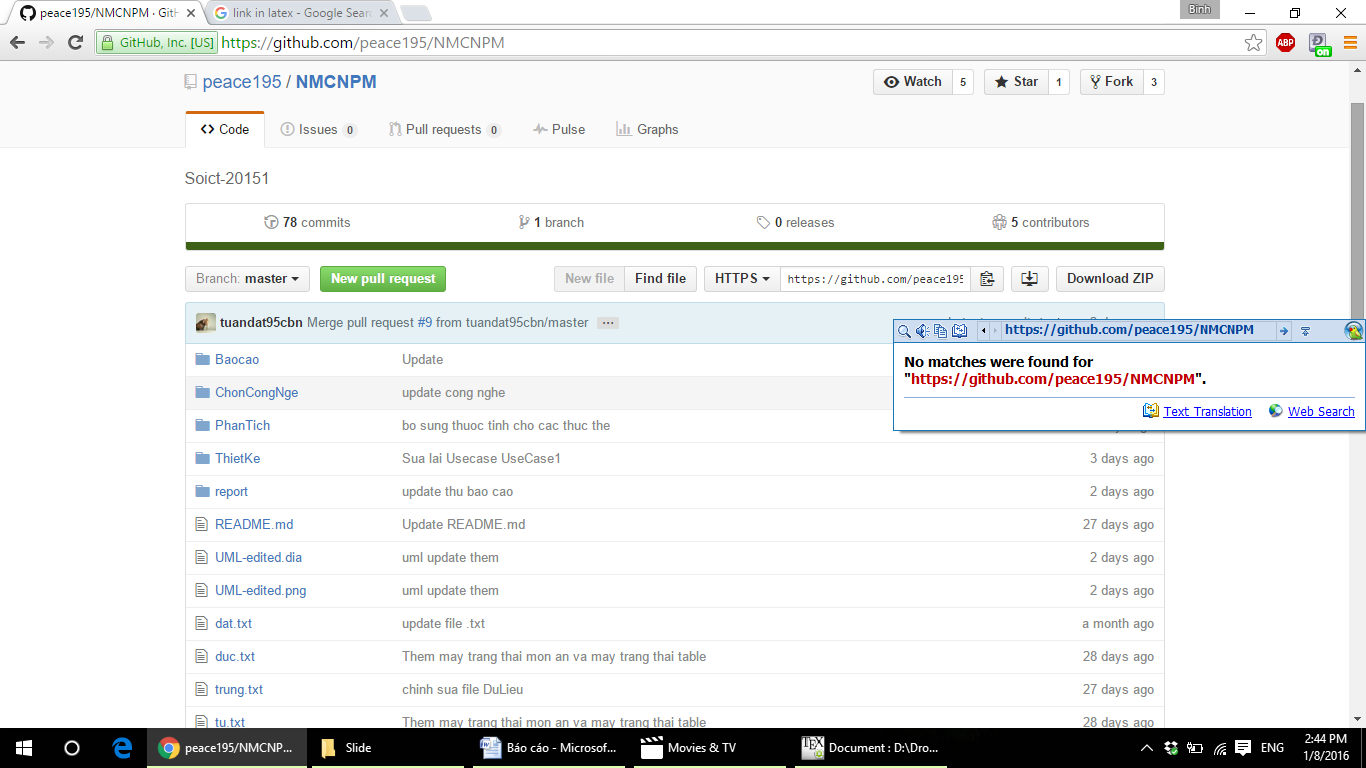
\includegraphics[scale=0.4]{vc1.png}\\
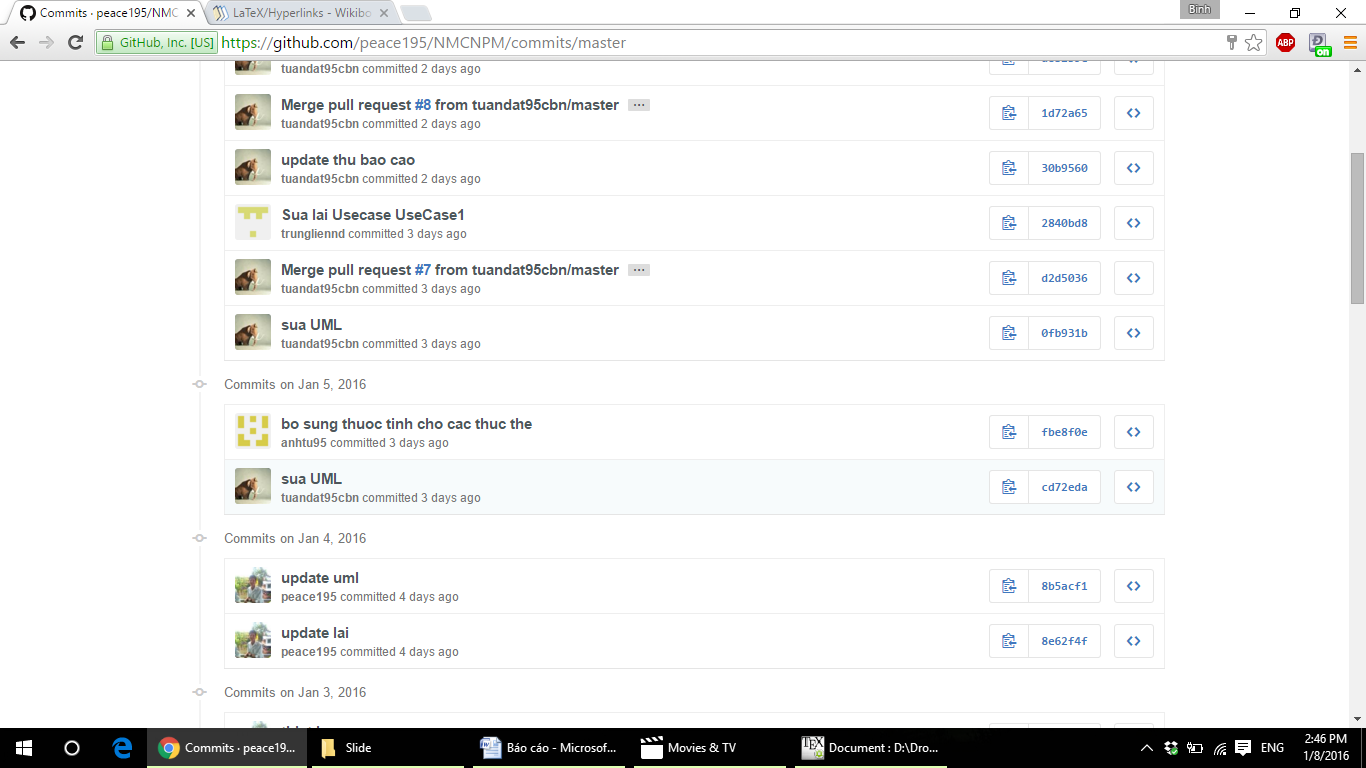
\includegraphics[scale=0.4]{vc2.png}
\end{center}
\chapter*{Tài liệu tham khảo}
\phantomsection
\addcontentsline{toc}{chapter}{Tài liệu tham khảo}
[1] Slide "Nhập môn công nghệ phần mềm", TS.Nguyễn Thanh Hùng
\end{document}